\documentclass[authoryear,11pt]{elsarticle}

%This eliminates the `Preprint submitted to...' footer on the first page
\makeatletter
\def\ps@pprintTitle{%
 \let\@oddhead\@empty
 \let\@evenhead\@empty
 \def\@oddfoot{}%
 \let\@evenfoot\@oddfoot}
\makeatother

\usepackage{amssymb}
\usepackage{amsthm}
\usepackage{caption}
\usepackage{amsmath}
\usepackage{morefloats}
\usepackage{bbm}        %To allow \mathbb{1}

\usepackage{rotating}   %To turn tables sidewaystable
\usepackage{graphicx}
\usepackage{setspace}
\usepackage{hyperref}

%\onehalfspacing

%\setlength{\parindent}{0pt}

\usepackage[top=3.5cm,bottom=3.75cm,left=2.45cm,right=2.45cm]{geometry}% by courtesy of Mico

\begin{document}
\begin{frontmatter}
\title{MFE Economics\\Problem set 4}
\end{frontmatter}

%%%%%%%%%%%%%%%%%%%%%%%%%%%%%%%%%%%%%%%%%%%%%%%%%%%%%%%%%%%%%%%%%%%%%%%%%%%%%%%%%%%%%%%%%%%%%%%%%%%%%%%%%%%%%%%%%%%%%%%%%%%%%%%%%%%%%%%%%%%%%%%%%%%%%%%%
%%%%%%%%%%%%%%%%%%%%%%%%%%%%%%%%%%%%%%%%%%%%%%%%%%%%%%%%%%%%%%%%%%%%%%%%%%%%%%%%%%%%%%%%%%%%%%%%%%%%%%%%%%%%%%%%%%%%%%%%%%%%%%%%%%%%%%%%%%%%%%%%%%%%%%%%

\section{New Keynesian Model - Price setting and Intuition}
As discussed in class and shown in the textbook (P. 60-63) we have
\begin{eqnarray}
\pi_{t} 			&=&	\beta E_{t}[ \pi_{t+1} ]	 - \lambda \hat{\mu}_{t}	 \label{eqn:mc_pc} \\
				&=&	\beta E_{t}[ \pi_{t+1} ]	 + \kappa \tilde{y_{t}}	\label{eqn:nkpc}
\end{eqnarray}
where
\begin{eqnarray*}
\lambda 			&\equiv& 	\theta^{-1}(1-\theta)(1-\beta\theta)\Theta > 0 \\
\Theta 			&\equiv& 	\frac{1-\alpha}{1-\alpha + \alpha \varepsilon} \\
\kappa			&\equiv&	\lambda \left(\sigma + \frac{\varphi + \alpha}{1-\alpha}  \right)
\end{eqnarray*}
and where
\begin{eqnarray*}
\hat{\mu}_{t} 	&\equiv&	 \mu_{t} - \mu \\
\mu_{t} 		&\equiv&	 p_{t} - \psi_{t} \\
\tilde{y}_{t}		&\equiv&	y_{t} - y^{n}_{t}
\end{eqnarray*}

\begin{itemize}
\item	Use equation (\ref{eqn:mc_pc}) to show that
\[
\pi_{t} = -\lambda \sum\limits_{k=0}^{\infty} \beta^{k} E_{t}[\hat{\mu}_{t+k}]
\]
HINT: Use equation (\ref{eqn:mc_pc}) in t+1 to get an expression for $\pi_{t+1}$ and substitute it into the (\ref{eqn:mc_pc}) on the RHS in the expectation, then use (\ref{eqn:mc_pc}) in t+2 in a similar way. Keep going and you'll see the pattern emerging. You'll have terms like $E_{t}[E_{t+1}[E_{t+2}\ldots]]]$. For this you will need to use the \href{https://en.wikipedia.org/wiki/Law_of_total_expectation}{`law of iterated expectations'} which means that $E_{t}[ E_{t+j}[ X ] ] = E_{t}[ X  ]$ for a random variable $X$ and $j\geq0$. Basically it means your expectation of `X' now (with your limited information available at $t$) of your expectation in the future of `X' (with greater information at $t+j$) is simply equal to your expectation now - which is intuitive. So $E_{t}[E_{t+1}[E_{t+2}\ldots]]]$ is just $E_{t}[\ldots]$
\item	Show that $\lambda$ is decreasing in the `Calvo parameter', $\theta$ and briefly discuss how a greater degree of price stickiness influences the value of inflation associated with a given expected path of markup deviations?\footnote{For this you will need to recall that
\[
\frac{d}{dx} f(x)g(x) = f'(x)g(x) + g'(x)f(x) \text{ and }\frac{d}{dx} \frac{f(x)}{g(x)} = \frac{f'(x)g(x)-g'(x)f(x)}{g(x)^{2}}
\]
}
\item	As discussed in class and shown in the textbook (P. 62) we have
\begin{eqnarray}
\mu_{t} &=& p_{t} - \psi_{t}	\nonumber \\
		&=& -(w_{t} - p_{t}) + (a_{t} - \alpha n_{t} + \log{(1-\alpha)}) \nonumber \\
		&=& -(\sigma y_{t} + \varphi n_{t}) + (a_{t} - \alpha n_{t} + \log{(1-\alpha)}) \nonumber\\
		&=& - \left( \sigma + \frac{\varphi + \alpha}{1-\alpha} \right)y_{t} + \left( \frac{1+\varphi}{1-\alpha} \right) a_{t} + \log{(1-\alpha)} \label{eqn:mu_eqn}
\end{eqnarray}
[HARDER - don't spend too long] Briefly give intuition for the dependence of the coefficient on $y_{t}$ in equation (\ref{eqn:mu_eqn}) on $\sigma$, $\varphi$ and $\alpha$. Hint: Note that the negative of the log markup is log real marginal cost. The intuition may be easier if you discuss the coefficient in terms of real marginal cost and its association with the output level\ldots
\[
mc_{t} \equiv \psi_{t} - p_{t}= \left( \sigma + \frac{\varphi + \alpha}{1-\alpha} \right)y_{t} - \left( \frac{1+\varphi}{1-\alpha} \right) a_{t} - \log{(1-\alpha)}
\]
\end{itemize}

\subsection*{Answers}
We start with the recursive relation in equation (\ref{eqn:mc_pc})
\begin{eqnarray*}
\pi_{t} 	&=& \beta E_{t}[ \pi_{t+1} ] - \lambda \hat{\mu}_{t} \\
		&=& \beta  E_{t}[ \beta E_{t+1}[ \pi_{t+2} ] - \lambda \hat{\mu}_{t+1} ] - \lambda \hat{\mu}_{t} \\
		&=& \beta^2  E_{t}[ E_{t+1}[ \pi_{t+2} ] ] - \lambda \beta E_{t}[ \hat{\mu}_{t+1} ] - \lambda \hat{\mu}_{t} \\
\end{eqnarray*}
Now we use the law of iterated expectations to obtain
\[
\pi_{t} 	= \beta^2  E_{t}[ \pi_{t+2}] - \lambda \beta E_{t}[ \hat{\mu}_{t+1} ] - \lambda \hat{\mu}_{t}
\]
Continuing, accordingly we can write this as
\begin{eqnarray*}
\pi_{t} 	&=&\beta^2  E_{t}[ \beta E_{t+2}[ \pi_{t+3} ] - \lambda \hat{\mu}_{t+2} ] - \lambda \beta E_{t}[ \hat{\mu}_{t+1} ] - \lambda \hat{\mu}_{t} \\
	&=& \beta^3  E_{t}[ \pi_{t+3}] - \lambda \beta^2 E_{t}[ \hat{\mu}_{t+2} ]- \lambda \beta E_{t}[ \hat{\mu}_{t+1} ] - \lambda \hat{\mu}_{t} \\
	&\ldots& \\
	&=& \beta^{J} E_{t}[ \pi_{t+J} ] - \lambda \sum\limits_{j=0}^{J-1} \beta^{j} E_{t}[ \hat{\mu}_{t+j} ]
\end{eqnarray*}
and since $\beta \in (0,1)$ and our inflation process is well behaved we obtain, as $J \to \infty$
\[
\pi_{t} = - \lambda \sum\limits_{j=0}^{\infty} \beta^{j} E_{t}[ \hat{\mu}_{t+j} ]
\]
since $\beta^{J} E_{t}[ \pi_{t+J} ] \to 0$ as $J\to \infty$.

Now, since $\Theta \in (0,1]$ and is a constant, to show that $\lambda$ is decreasing in $\theta$ we need only show that
\[
\frac{(1-\theta)(1-\beta\theta)}{\theta}
\]
is decreasing in $\theta$.

If we take the derivative with respect to $\theta$ (using the rules in the footnote in the question) we obtain
\[
\frac{(-(1-\beta \theta)-\beta(1-\theta)) - (1-\theta)(1-\beta \theta)}{\theta^{2}}
\]
which is proportional to the numerator, as $\theta^2 > 0$. Thus we need to show that the numerator is negative. If we rearrange it, then we find that it is equal to $\beta \theta^2 - 1$ which is negative since $\beta$ and $\theta$ are both assumed to be positive and less than $1$.

The insight that, for a given expected path of deviations of markups from desired, the change in the price level is less extreme, may initially seem obvious. $\theta$ being larger naturally suggests more inertia, all else equal, since fewer firms can change prices in a given period. Note however, that it is not \emph{completely} obvious \emph{a priori} as one might have wondered if, in equilibrium, the changes made by the firms that \emph{can} reset their prices might be larger to `compensate' for a larger $\theta$ - possibly to the extent that the net effect would be to make the change in the price level bigger for a given expected path of markups. However, it turns out that is not the case here.

Note that the definition of $\kappa$ in the New Keynesian Phillips curve means that a lower $\lambda$ arising from a higher $\theta$ makes the slope of the Phillips curve `flatter'. The (apparent) flattening of the Phillips curve relationship has been a matter of intense debate in recent years (in the context of statistical models and much richer structural New Keynesian models).\footnote{One implication of a flattening Phillips Curve is, to the extent monetary policy is thought to operate on inflation via its impact on activity, more dramatic shifts policy are required to influence the price level since they must induce more dramatic effects on activity (note this argument is often very loose and frequently takes a `non-equilibrium' flavor in the sense of ignoring what shocks might have caused the lack of co-movement.). Additionally, a flattening Phillips Curve has been suggested as a reason why dramatic real weakness in the last recession did not result in as low inflation as pre-crisis models would have suggested (again, these arguments are often made very loosely).}

Turning to the coefficient on $y_{t}$ in equation (\ref{eqn:mu_eqn}) we first note that (as mentioned in the hint) $-\mu_{t}$ is equal to (log) real marginal cost. The discussion below is most natural if we explain the association between marginal cost and output. Thus
\[
mc_{t} \equiv \psi_{t} - p_{t}= \left( \sigma + \frac{\varphi + \alpha}{1-\alpha} \right)y_{t} - \left( \frac{1+\varphi}{1-\alpha} \right) a_{t} - \log{(1-\alpha)}
\]

Let us first consider it under the assumption of constant returns to scale in the production technology ($\alpha=0$).\footnote{All the statements below take $a_{t}$ as given. Note that it may be a shock to $a_{t}$ that drives changes in $y_{t}$ (and $\mu_{t}$).} In that case the coefficient simply reflects the household's intratemporal optimality condition (where this has entered via the wage's role in marginal cost) plus the fact that we have substituted $y_{t}$ for $c_{t}$. These two elements reflect two features of equilibrium - optimality and market clearing. The higher is $\varphi$ the more an additional hour costs a household in disutility. Thus to obtain the greater labor supply associated with greater output, the wage must be higher (raising marginal cost, all else equal).

Similarly, if $\sigma$ increases, the marginal utility of consumption is, all else equal, reduced, implying that the value of an additional hour to the household is reduced on the margin (since the consumption purchased with the additional wages yields less utility). Again, all else equal, the wage - and thus the marginal cost - must increase more within any increase in output. Note that we aren't making causal statements - these are simply statements about associations between variables that must hold in equilibrium.

Interestingly, in equilibrium, there is an association between marginal cost and the scale of output (for a given $a_{t}$) even if there are constant returns to scale ($\alpha=0$). Under a constant returns to scale assumption, from the perspective of an individual price taking firm, marginal cost is independent of their scale of production since they treat the wage as given and marginal product of labor is simply $A_{t}$ (recall, marginal cost is wage over marginal product of labor). The positive association arises in equilibrium however because wages must adjust in equilibrium in order to make the changed level of output consistent with optimal labor supply decisions by the household. If there are \emph{decreasing} returns to scale ($\alpha>0$), marginal cost is not constant with scale from the firm's perspective - it is positively related to scale - and this feeds through in the aggregate also. Hence $\alpha$ appearing in the coefficient on $y_{t}$.

\section{DIS and NKPC}
The dynamic IS curve (DIS) and the New Keynesian Phillips curve (NKPC) are given by
\begin{eqnarray*}
y_{t} &=& E_{t}[y_{t+1}] - \frac{1}{\sigma}(i_{t} - E_{t}[\pi_{t+1}] - \rho) + \frac{1}{\sigma}(1-\rho_{z})z_{t} \\
\pi_{t} &=& \beta E_{t}[ \pi_{t+1} ] + \kappa \tilde{y}_{t}
\end{eqnarray*}

First we will consider the DIS curve and go through a few thought experiments to investigate some of its properties.
\begin{itemize}
\item	Sketch a plot of the DIS with $y_{t}$ on the horizontal axis and $i_{t}$ on the vertical axis (rearrange the DIS to have $i_{t}$ on the LHS and then sketch - don't worry about exact numbers, but generally people think $\sigma$ is a positive number greater than $1$ and $\beta$ is something like $0.99$.)
\item	What is the slope? Give intuition in a sentence or two.
\end{itemize}
Note that implicitly the location of the curve depends on assumed values for the structural parameters ($\sigma$, $\rho_{z}$ and $\rho \equiv -\log{(\beta)}$), the other endogenous variables that feature in the DIS ($E_{t}[y_{t+1}]$, $E_{t}[\pi_{t+1}]$) and the preference shock ($z_{t}$). Recall, also, that in our simple model $y_{t}=c_{t}$ (in richer models it might also feature investment and government expenditure).
\begin{itemize}
\item	What happens to the curve in the following situations? Give intuition.
	\begin{itemize}
	\item	Suppose something shifts $E_{t}[y_{t+1}]$ up (and increase in confidence about the future, say), holding all else equal.
	\item	Suppose something shifts $E_{t}[\pi_{t+1}]$ up (some inflationary expectations pick up), holding all else equal.
	\item	What if $z_{t}$ increases, holding all else equal.
	\item	What if $\beta$ increases, or $\sigma$?
	\end{itemize}
\item	In a few sentences, why is `holding all else equal' an unnatural assumption in this context?
\item	Redraw the DIS but now with the real interest rate on the vertical axis
	\begin{itemize}
	\item	Suppose, again, something shifts $E_{t}[\pi_{t+1}]$ up, holding all else equal. What movement is associated with this, now that we have re-drawn the DIS? Is it a curve shift? Comment briefly.
	\end{itemize}
\end{itemize}
Now we turn to the NKPC and consider some more thought experiments. Think about plotting it in $(\tilde{y}_{t},\pi_{t})$ space (sketch it if you want)
\begin{itemize}
\item	What happens to the curve in the following situations? Give intuition.
	\begin{itemize}
	\item	What happens if something shifts $E_{t}[\tilde{y}_{t+2}]$ up, holding all else equal (again, an unnatural assumption). Give intuition in a couple of sentences.
	\item	What if $\theta$ increases, or $\varphi$? Give intuition in a couple of sentences.
	\end{itemize}
\end{itemize}

\subsection*{Answers}
Before we get going on answering this question I just want to point out that `shifting curves' is a very popular way of learning in undergraduate economics but, in my opinion, it is problematic. The DIS curve offers a good example (setting aside the `unnatural' aspect of holding all else equal in equilibrium - see later part of question).

The DIS involves various endogenous variables, not just $i_{t}$ and $y_{t}$. Specifically, it involves $E_{t}[y_{t+1}]$ and $E_{t}[\pi_{t+1}]$, which are no less a part of the DIS than $i_{t}$ and $y_{t}$. Really, if we could draw in four (or, five, including $z_{t}$) dimensions we could completely sketch the DIS and then, when considering the first two `curve shifting' experiments below, we would see that nothing is actually shifting - the relationship among all the variables is unchanged. Instead, when we choose to look at the relationship in 2-D space we can only look at a slice of the overall plot of the relationship - i.e. the relationship between $i_{t}$ and $y_{t}$ for a particular pair of $E_{t}[y_{t+1}]$ and $E_{t}[\pi_{t+1}]$. The first two experiments below are simply a question of looking at different slices - and in 2-D that looks like a curve shift.

If we wanted to imagine a 5-D relationship (adding $z_{t}$ into the mix) then the same sort of logic applies, as discussed above. When it comes to changes in the deep parameters, though, I think it is fair to think of the relationship changing - and the 5-D association between $i_{t}$, $y_{t}$, $E_{t}[y_{t+1}]$, $E_{t}[\pi_{t+1}]$ and $z_{t}$ being `shifted' (though of course this is just a matter of taste, you could imagine an 8-D surface with axes for the parameters too - though that doesn't seem natural). Anyway\ldots

As shown on the left hand side of figure \ref{fig:dis_nkpc} below, the DIS is a downward sloping relation in $(y_{t},i_{t})$ space with slope $-\sigma$. Now, in terms of the experiments\ldots
\begin{itemize}
\item	If there is an increase in $E_{t}[y_{t+1}]$ then the curve `shifts' (remember the previous discussion though) rightwards - i.e. at any given $i_{t}$, $y_{t}$ will be higher. The intuition is that the consumer's optimality condition (on which this curve is effectively based since $c_{t}=y_{t}$ in equilibrium) reflects a desire for consumption smoothing.
\item	Higher expected inflation, for any given $i_{t}$ implies a lower real interest rate - this makes consumption today more desirable, relative to consumption tomorrow (\textbf{which is being held equal}), so the curve shifts rightwards. In fact, it is perhaps more natural to think of it shifting vertically as now, a higher nominal interest rate is associated with a given $y_{t}$ since that higher $i_{t}$, combined with the higher $E_{t}[\pi_{t+1}]$ yields the same $r_{t}$ that was previously associated with that value of $y_{t}$ (holding the other elements of the DIS constant).
\item	If $z_{t}$ increases, all else equal, then it is as if the household becomes more impatient (recall, a higher $z_{t}$ shows up a bit like a lower $\beta$) so that they want to pull consumption forward to the present. Hence there is more demand in the current period for a given $i_{t}$ (or for a given $r_{t}$, which, since inflation expectations are being held fixed, is equivalent to a given $i_{t}$), which looks like a rightward shift in the the DIS, in $(y_{t},i_{t})$ space.
\item	A higher $\beta$ (as the previous answer suggests) would imply a leftward shift in the curve (less demand for current consumption relative to future consumption - which is being held fixed) for a given $i_{t}$ due to the household's increased patience. Note that you need to recall that $\rho$ is a transformed version of $\beta$. A change in $\sigma$ actually changes the slope of the line in $(y_{t},i_{t})$ space so that the slope becomes steeper (more steeply downward sloping). Recall that $\sigma^{-1}$ is the elasticity of intertemporal substitution (i.e. how willing the agent is to substitute consumption over time in response to a change in the market terms of trade). The more willing you are to substitute (the larger is $\sigma^{-1}$, or the smaller is $\sigma$) the smaller a change in $i_{t}$ is required for (or will be associated with) a given change in $c_{t}$, which in this case is equal to $y_{t}$.
\end{itemize}

Why is `holding all else equal' unnatural in this context? We are only working with one of the equations that implicitly defines the equilibrium values of the endogenous variables in terms of the underlying state. In equilibrium, we use this and other (e.g. market clearing relations, the NKPC, the Taylor rule,\ldots) to solve explicitly for the functions relating the endogenous variables to the state. The endogenous variables do not have direct causal influences on eachother (without making additional assumptions) and, most relevantly for this question, when they move, it must be because of some change in the underlying state. Generally, if one endogenous variable is changing (such as the changes considered in our questions) the state that is implicitly driving that change will, in equilibrium, also be changing the other variables. Thus, it is a bit unnatural to assume they \emph{don't} change (which is what we mean by `holding all else equal').

In the middle of figure \ref{fig:dis_nkpc} we see the DIS curve re-written in $(r_{t},y_{t})$ space, where we recall $r_{t} = i_{t} - E_{t}[\pi_{t+1}]$. It looks pretty much as before - downward sloping with slope $-\sigma$. Note that once we re-express DIS explicitly in terms of $r_{t}$ a change in inflation expectations, all else equal, is like a movement along the curve rather than a shift in the curve since it changes $r_{t}$ for a given $i_{t}$ where the latter is held fixed.

Now, turning to the NKPC, the right hand side of figure \ref{fig:dis_nkpc} shows that it is an upward sloping relations, with slope $\kappa$. Recall that $\kappa$ is defined as follows
\begin{eqnarray*}
\lambda 			&\equiv& 	\theta^{-1}(1-\theta)(1-\beta\theta)\Theta > 0 \\
\Theta 			&\equiv& 	\frac{1-\alpha}{1-\alpha + \alpha \varepsilon} \\
\kappa			&\equiv&	\lambda \left(\sigma + \frac{\varphi + \alpha}{1-\alpha}  \right)
\end{eqnarray*}

Now, what if $E_{t}[\tilde{y}_{t+2}]$ increases, holding all else equal? Note that $E_{t}[\tilde{y}_{t+2}]$ doesn't figure explicitly but recall that we can re-express the relation as
\[
\pi_{t} = \kappa \sum\limits_{k=0}^{\infty} \beta^{k} E_{t}[ \tilde{y}_{t+k} ]
\]
so we see that there will be a rightward shift in the curve, or perhaps it is more natural to think of it as an upward shift. Future output gap is expected to be higher and, thus, future marginal costs are expected to be higher, all else equal, so firms setting their prices today anticipate this (recall they are forward looking due to the fact the price they set today may prevail for several periods) and raise their prices more then they otherwise would have given the \emph{current} output gap, implying higher inflation (hence the `shift' upwards). The next part of the question is pretty much the same but the shift will be smaller for a given change in future expected output gap because it is weighted by $\kappa \beta^{3} < \kappa \beta^{2}$. Again, holding everything else equal is somewhat unnatural in this context, perhaps most obviously because any news today that the output gap will (in expectation) be higher in two (or three) periods' time will `likely' imply that expectations of the output gap will shift at other horizons too.

Regarding changes in parameters, as discussed in the previous homework, an increase in $\theta$ lowers $\lambda$ and thus flattens the slope of the curve. In contrast, increasing $\varphi$ steepens the Phillips curve.

\begin{figure}[!htb]
\center{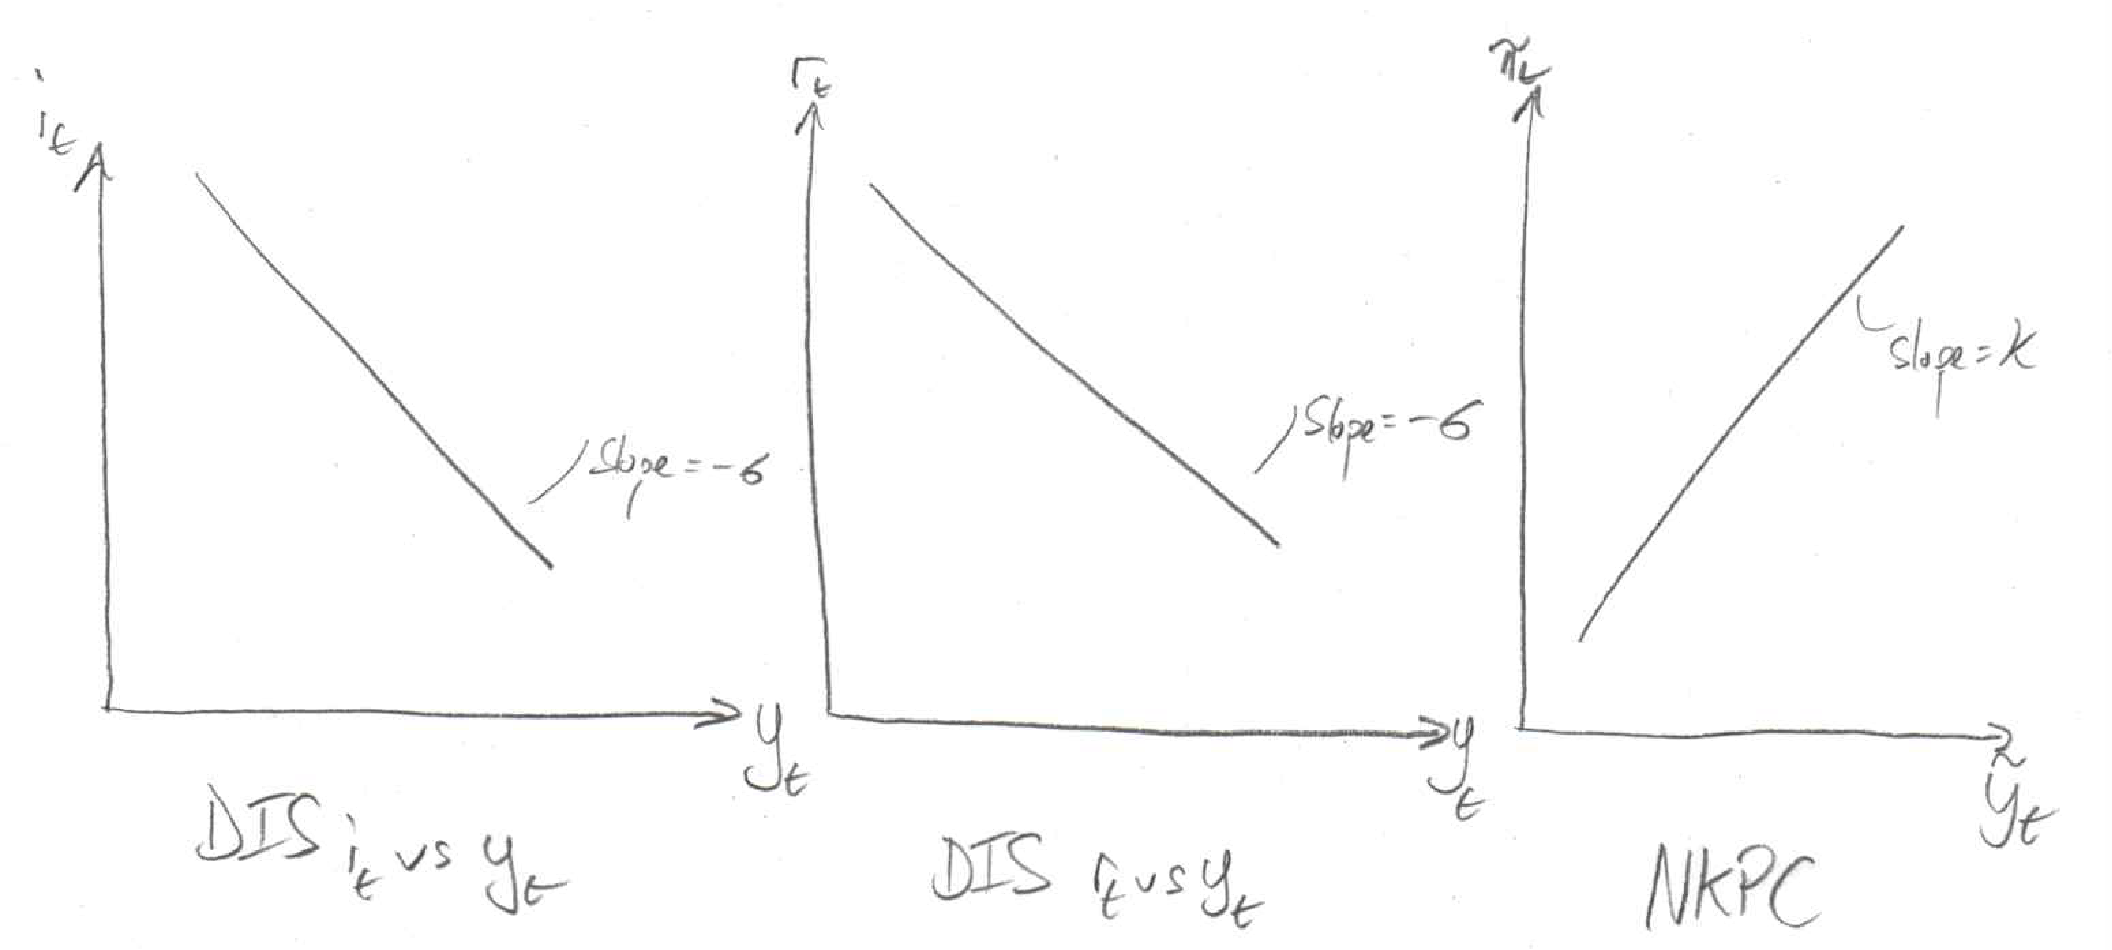
\includegraphics[width=1.0\textwidth]{dis_nkpc_figure.pdf}}
\caption{\label{fig:dis_nkpc} Sketch Dynamic IS and New Keynesian Phillips Curves}
\end{figure}

\section{Useful prep for next lecture (try it and then come back after the lecture): Autoregressive processes}
In the models we consider, there are random `shock' or `driving' processes that are exogenous to the model.\footnote{You can brush up on random variables \href{https://en.wikipedia.org/wiki/Random_variable}{here}, on Normal variables \href{https://en.wikipedia.org/wiki/Normal_distribution}{here} and on expected value (or `the mean') \href{https://en.wikipedia.org/wiki/Expected_value}{here}.} In our case these shocks (technology, time preference and monetary policy) will constitute the `state' of the economy in the sense that all the endogenous variables (consumption, output, wages, interest rates) will in equilibrium be expressible as functions of these three variables (or subsets thereof, depending on the model). All the shocks we consider, when logged, follow an autoregressive process of order $1$ or, for short, an $AR(1)$. Consider the technology shock $A_{t}$ from the production function $Y_{t} = A_{t}N_{t}^{1-\alpha}$. When expressed in logs it follows this process\footnote{Note that is convenient to model it this way as it means that $A_{t}$, while random, will always be positive (as makes sense for a technology term that multiplies - some function of - labor to produce non-negative output). Frequently in economics or finance we use the exponential of a random variable to obtain a transformed random variable that is positive. In fact, exponentials have other nice properties when working with Normal distributions.}
\begin{eqnarray}
a_{t} 			&=& \rho_{a} a_{t-1} + \varepsilon_{a,t} 	\label{eqn:ar1} \\
\varepsilon_{a,t} &\overset{iid}{\sim}& N(0,\sigma^{2}_{a})	\nonumber \\
a_{t}			&\equiv& \log{(A_{t})} \nonumber
\end{eqnarray}

The random variable, $\varepsilon_{a,t}$  (what I will often refer to as an `innovation'), is a Gaussian or `Normal' variable with zero mean ($E_{t}[\varepsilon_{a,t+1}] = 0$) and variance, $\sigma^{2}_{a}$ ($E_{t}[(\varepsilon_{a,t+1} - 0)^{2}] = \sigma^{2}_{a}$). It is also independently and identically distributed (iid) which means that there is no dependence between its draws in different periods or between its draw and any other variables and the distribution from which it is drawn ($N(0,\sigma^{2}_{a})$) is constant over time. The parameter $\rho_{a}$ will be referred to as a `persistence' parameter. We will always (in this course) consider cases where $|\rho_{a}| \in (0,1)$ - in the language of stochastic processes, this ensures that it is a `stationary' process.

\begin{itemize}
\item	Show that\footnote{HINT: Use equation (\ref{eqn:ar1}) but for earlier periods ($a_{t-1}$, $a_{t-2}$ etc.) to repeatedly replace the lagged values of $a_{t}$ on the right hand side of equation (\ref{eqn:ar1}). This is a bit like the first part of the first question above - but you're now going back in time rather than forwards.}
\begin{equation}
a_{t} = \sum\limits_{j=0}^{J-1} \rho_{a}^{j} \varepsilon_{a,t-j} + \rho_{a}^{J} a_{t-J} \label{eqn:sum_ar}
\end{equation}
\end{itemize}

Suppose data started in $t=0$, so that $a_{0}$ is just given to us, then we just set $J=t$ in the above expression. If there is no explicit starting point then we can use the assumption on $|\rho_{a}| \in (0,1)$ to state
\[
a_{t} = \sum\limits_{j=0}^{\infty} \rho_{a}^{j} \varepsilon_{a,t-j}
\]
since $\rho_{a}^{J} a_{t-J} \to 0$ as $J \to \infty$. Intuitively, if the effects of shocks dies of to zero in the limit - and given that our shocks are well behaved - we can ignore the last term in expression (\ref{eqn:sum_ar}) you just derived because it gets arbitrarily small.

\begin{itemize}
\item	What is the effect of an innovation $j$ periods ago on $a_{t}$ (i.e. the effect of $\varepsilon_{a,t-j}$)?
\item	What is the effect of an innovation in $t$ on $a_{t+1}$? On $a_{t+2}$? On $a_{t+j}$?
\end{itemize}

Any effect an innovation in $t$ has on future values of $a_{t}$, say $a_{t+j}$,  may be flooded by the effects of future innovations in later periods before period $t+j$. But it is still useful to talk about the effect the innovation has as this nevertheless does \emph{contribute} to $a_{t+j}$ (look back at the expression you derived above - $a_{t}$ is made up of a weighted sum of all current and previous innovations, with those weights declining as the innovation period recedes into the distant past). Given the process we are considering and the iid assumptions made on $\varepsilon_{a,t}$, an innovation today does affect the expected value - from the perspective of today - of future values of the technology shock.\footnote{To answer questions involving expectations below, recall that the expectations operator is linear (in particular, that means $E_{t}[X + Y] = E_{t}[X] + E_{t}[Y]$), the expectation of a constant (or something already known when the expectation is being formed) is the constant itself and the expectation of a scalar constant times a random variable is the scalar constant times the expectation of the random variable.}

\begin{itemize}
\item	What is the expected value of $a_{t+1}$ given information available in $t$ (i.e. given you know $a_{t}$)?
\item	What is the expected value of $a_{t+2}$ given information available in $t$
\item	What is the expected value of $a_{t+j}$ given information available in $t$
\item	What is the expected value of $\Delta a_{t+1} \equiv a_{t+1} - a_{t}$ given information available in $t$
\item	How does today's ($t$) innovation affect your expectation of $a_{t+j}$ relative to the expectation you held in $t-1$ before you knew $\varepsilon_{a,t}$?
\end{itemize}

%In the models we consider we will often express the equilibrium values of endogenous variables as functions of $a_{t}$ (and other shocks). Suppose a variable $s_{t}$ is expressed
%\[
%s_{t} = \psi_{0} + \psi_{1} a_{t}
%\]
%\begin{itemize}
%\item	What is $s_{t+1}$ in terms of $a_{t+1}$?
%\item	What is $s_{t+1}$ in terms of $a_{t}$ and $\varepsilon_{a,t+1}$?
%\item	What is the expected value of $s_{t+1}$ given information available in $t$ (i.e. given you know $a_{t}$)?
%\item	What is the expected value of $\Delta s_{t+1} \equiv s_{t+1} - s_{t}$ given information available in $t$
%\end{itemize}

\subsection*{Answers}
By repeatedly lagging and substituting the equation (\ref{eqn:ar1}) we get (in what follows I just write $\rho$ and $\varepsilon_{t}$ instead of  $\rho_{a}$ and $\varepsilon_{a,t}$
\begin{eqnarray*}
a_{t} 	&=&	\rho a_{t-1} + \varepsilon_{t} \\
		&=&	\rho(\rho a_{t-2} + \varepsilon_{t-1}) + \varepsilon_{t} \\
		&=&	\rho(\rho(\rho a_{t-3} + \varepsilon_{t-2}) + \varepsilon_{t-1}) + \varepsilon_{t}	\\
		&\ldots& \sum\limits_{j=0}^{J-1} \rho^{j} \varepsilon_{t-j} + \rho^{J}a_{t-J}
\end{eqnarray*}

Since we have $\rho^{J}a_{t-J} \to 0$ as $J \to \infty$ we have $a_{t} = \sum\limits_{j=0}^{\infty} \rho^{j} \varepsilon_{t-j}$ so that the effect of $\varepsilon_{t-j}$ on $a_{t}$ is $\rho^{j} \varepsilon_{t-j}$. So if $\varepsilon_{t-j}=1.7$ the contribution is $1.7\rho^{j}$. With similar logic, the effects of an innovation in $t$ on $a_{t+1}$, $a_{t+2}$ and $a_{t+j}$ are $\rho \varepsilon_{t}$, $\rho^{2} \varepsilon_{t}$ and $\rho^{j} \varepsilon_{t}$, respectively.

The expected value of $a_{t+1}$ given information in $t$ is
\[
E_{t}[a_{t+1}] = E_{t} [ \rho a_{t} + \varepsilon_{t+1} ] = E_{t} [ \rho a_{t} ] + E_{t}[ \varepsilon_{t+1} ] = \rho a_{t}  + 0 = \rho a_{t}
\]

The expected value of $a_{t+2}$ given information in $t$ is
\[
E_{t}[a_{t+2}] = E_{t} [ \rho a_{t+1} + \varepsilon_{t+2} ] = E_{t} [ \rho a_{t+1} ] + E_{t}[ \varepsilon_{t+2} ] = \rho E_{t}[a_{t+1}]  + 0 = \rho^2 a_{t}
\]

The expected value of $a_{t+2}$ given information in $t$ is, by induction, $\rho^{j} a_{t}$ or, explicitly, by using equation (\ref{eqn:sum_ar}) applied to $a_{t+j}$
\[
E_{t}[a_{t+j}] = E_{t}[ \sum\limits_{k=0}^{j-1} \rho^{k} \varepsilon_{t+j-k} + \rho^{j} a_{t} ] = \rho^{j} a_{t} + \sum\limits_{k=0}^{j-1} \rho^{k} E_{t}[\varepsilon_{t+j-k}] =  \rho^{j} a_{t}
\]

The expected change in technology is given by
\[
E_{t}[\Delta a_{t+1} \equiv E_{t}[ a_{t+1} - a_{t}] = \rho a_{t} - a_{t} = (\rho - 1) a_{t}
\]
or you could equivalently think of this as
\[
E_{t}[\Delta a_{t+1} \equiv E_{t}[ a_{t+1} - a_{t}] =  \equiv E_{t}[ (\rho-1) a_{t} + \varepsilon_{t+1}] = (\rho - 1) a_{t}
\]

Suppose you receive news (in the form of $\varepsilon_{t}$) between period $t-1$ and $t$. How would that change your expectation of $a_{t+j}$? Let us compare the following two expectations (look carefully at the first one and make sure you understand)
\begin{eqnarray*}
E_{t-1}[ a_{t+j} ] = \rho^{j+1} a_{t-1}	\\
E_{t} [ a_{t+j} ] = \rho^{j} a_{t}
\end{eqnarray*}
But the second can be re-expressed as $\rho^{j+1} a_{t-1} + \rho^{j} \varepsilon_{t}$ and thus
\[
E_{t} [ a_{t+j} ] - E_{t-1}[ a_{t+j} ] = \rho^{j}  \varepsilon_{t}
\]
Sometimes we use the notation $\Delta E_{t}[ a_{t+j} ] \equiv E_{t} [ a_{t+j} ] - E_{t-1}[ a_{t+j} ]$ to denote the effect of news but this notation can be a bit confusing. The $\Delta$ refers to change in the expectation, not in $a_{t+j}$.
%
%Finally, turning to variable $s_{t}$ we have in terms of $a_{t+1}$ or in terms of $a_{t}$ and $\varepsilon_{t+1}$
%\begin{eqnarray*}
%s_{t+1} &=& \Psi_{0} + \Psi_{1} a_{t+1}	\\
%s_{t+1} &=& \Psi_{0} + \rho \Psi_{1} a_{t} + \Psi_{1} \varepsilon_{t+1}
%\end{eqnarray*}
%
%The expected value of $s_{t+1}$ given $t$ information is
%\[
%E_{t}[s_{t+1}] = E_{t}[ \psi_{0} + \psi_{1} a_{t+1} ] = \psi_{0} + \psi_{1} E_{t}[ a_{t+1}] = \psi_{0} + \psi_{1} \rho a_{t}
%\]
%
%And the expected change in $s_{t+1}$ is
%\[
%E_{t}[ \Delta s_{t+1} ] = E_{t}[  \psi_{0} + \psi_{1} a_{t+1}  -  \psi_{0} - \psi_{1} a_{t} ] = \psi_{1} E_{t}[\Delta a_{t+1}] = \psi_{1} (\rho-1) a_{t}
%\]

\section{Optional/Hard: Optimal price setting and practice linearization}
Use a first order approximation of
\begin{equation}
\sum\limits_{k=0}^{\infty} \theta^{k} E_{t} \left[ \Lambda_{t,t+1} Y_{t+k|t} \frac{1}{P_{t+k}} \left( P_{t}^{\ast} - \mathcal{M}\Psi_{t+k|t} \right) \right] = 0\label{eqn:fwd_obj_fn}
\end{equation}
around the zero inflation steady state, to obtain (as claimed in the text p. 57 2nd ed.)
\[
p_{t}^{\ast} = \mu + (1-\beta \theta) \sum\limits_{k=0}^{\infty}(\beta \theta)^{k} E_{t}[\psi_{t+k|t}]
\]

\subsection*{Answers}
We define $\Omega_{t,t+k}\equiv \frac{1}{\beta^{k}} \Lambda_{t,t+k}$ (noting that $\Omega_{t,t+k}=1$ in steady state, for all $k$) and rewrite equation (\ref{eqn:fwd_obj_fn}) as\footnote{$\Omega_{t,t+k}=1$ in steady state, for all $k$ since consumption is constant in steady state, $\Lambda_{t,t+k}\equiv \beta^{k} \frac{U_{c,t+k}}{U_{c,t}}$ and we have taken out the $\beta$ element of the multi-step SDF in defining $\Omega$.}
\[
\sum\limits_{k=0}^{\infty} (\beta \theta)^{k} E_{t} \left[ \Omega_{t,t+1} Y_{t+k|t} \frac{1}{P_{t+k}} \left( P_{t}^{\ast} - \mathcal{M}\Psi_{t+k|t} \right) \right] = 0
\]
We the re-express in terms of log versions (lower case) of the variables in preparation for linearization in terms of the log variables
\[
\sum\limits_{k=0}^{\infty} (\beta \theta)^{k} E_{t} \left[ e^{\omega_{t,t+k} + y_{t+k|t} - p_{t+k}} \left( e^{p_{t}^{\ast}} - e^{\mu + \psi_{t+k|t}} \right) \right] = 0
\]
where $\mu \equiv \log{(\mathcal{M})}$ is the log `desired' or `flexible price' markup.

Now, note that in steady state $P_{t}-\mathcal{M} \Psi_{t+k|t}$ (in the steady state, the desired markup holds) - so the steady state of the term $\left( e^{p_{t}^{\ast}} - e^{\mu + \psi_{t+k|t}} \right)$ is $0$. Let us also call the steady state of the term  $e^{\omega_{t,t+k} + y_{t+k|t} - p_{t+k}}$, $\zeta$, which is $>0$. Then we can take a first order approximation and obtain
\[
0 \approx \sum\limits_{k=0}^{\infty} (\beta \theta)^{k} E_{t} \left[ \zeta \left( (p_{t}^{\ast} - \bar{p}^{\ast}) e^{\bar{p}^{\ast}} - (\psi_{t+k|t} - \bar{\psi}) e^{\mu + \bar{\psi}} \right) \right]
\]
but since $\zeta>0$ we can divide through and get
\begin{eqnarray*}
0 &\approx& \sum\limits_{k=0}^{\infty} (\beta \theta)^{k} E_{t} \left[ \left( (p_{t}^{\ast} - \bar{p}^{\ast}) e^{\bar{p}^{\ast}} - (\psi_{t+k|t} - \bar{\psi}) e^{\mu + \bar{\psi}} \right) \right] \\
 &=& \sum\limits_{k=0}^{\infty} (\beta \theta)^{k} E_{t} \left[ \left( p_{t}^{\ast} e^{\bar{p}^{\ast}} - \psi_{t+k|t}e^{\mu + \bar{\psi}} - \bar{p^{\ast}} e^{\bar{p}^{\ast}} + \bar{\psi}e^{\mu + \bar{\psi}}\right) \right] \\
 &=& \sum\limits_{k=0}^{\infty} (\beta \theta)^{k} E_{t} \left[ \left( p_{t}^{\ast} e^{\bar{p}^{\ast}} - \psi_{t+k|t}e^{\bar{p}^{\ast}} - \bar{p^{\ast}} e^{\bar{p}^{\ast}} + \bar{\psi}e^{\bar{p}^{\ast}}\right) \right]
\end{eqnarray*}
where in the last line we also used the fact that $\bar{p}^{\ast} = \mu + \bar{\psi}$ (this is just the steady state markup relation). Now we can divide through by $e^{\bar{p}^{\ast}}$ to obtain
\begin{eqnarray*}
0 &\approx& \sum\limits_{k=0}^{\infty} (\beta \theta)^{k} E_{t} \left[ \left( p_{t}^{\ast} - \psi_{t+k|t} - \bar{p^{\ast}} + \bar{\psi} \right) \right] \\
 &=& \sum\limits_{k=0}^{\infty} (\beta \theta)^{k} E_{t} \left[ p_{t}^{\ast} - \psi_{t+k|t} - \mu \right] 
\end{eqnarray*}
where we used the definition of the log markup. Now we are almost done as we simply need to rearrange. Specifically, we have
\[
 \sum\limits_{k=0}^{\infty} (\beta \theta)^{k} E_{t} \left[ p_{t}^{\ast} - \mu \right]  \approx \sum\limits_{k=0}^{\infty} (\beta \theta)^{k} E_{t} \left[ \psi_{t+k|t} \right] 
\]
but the terms on the LHS are known at $t$ so we can drop the expectation operator and, recalling that $\sum\limits_{k=0}^{\infty} (\beta \theta)^{k} = (1-\beta \theta)^{-1}$ (since $\beta \theta \in (0,1)$) we get
\[
 \frac{p_{t}^{\ast} - \mu}{1-\beta \theta}  \approx \sum\limits_{k=0}^{\infty} (\beta \theta)^{k} E_{t} \left[ \psi_{t+k|t} \right] 
\]
or, finally, as required
\[
p_{t}^{\ast} \approx  \mu + (1-\beta \theta) \sum\limits_{k=0}^{\infty} (\beta \theta)^{k} E_{t} \left[ \psi_{t+k|t} \right] 
\]
So that price is a markup of a particular weighted average of current and future marginal costs.

\end{document}

